\documentclass[10pt,a4paper]{article}
\usepackage[margin=2.05cm]{geometry}
\usepackage[T1]{fontenc}
\usepackage{lmodern}
\usepackage{microtype}
\usepackage{graphicx}
\usepackage{booktabs}
\usepackage{longtable}
\usepackage{array}
\usepackage{amsmath}
\usepackage{xcolor}
\usepackage[hidelinks]{hyperref}
\usepackage{enumitem}
\usepackage{fancyhdr}
\usepackage{float}
\graphicspath{{figures/}}
\definecolor{accent}{HTML}{1D4ED8}
\hypersetup{colorlinks=true,linkcolor=accent,urlcolor=accent,citecolor=accent}
\pagestyle{fancy}
\fancyhf{}
\setlength{\headheight}{14pt}
\setlength{\headsep}{18pt}
\lhead{Neural MS2LDA mean-evidence experiment}
\rhead{Seed 42, K=1000, six CPU threads}
\cfoot{\thepage}
\setlist{nosep,leftmargin=*}
\title{Mean token-type evidence closes the seed-42 neural MS2LDA annotation gap}
\author{MS2LDA research checkpoint}
\date{22 August 2026}

\begin{document}
\maketitle

\begin{abstract}
We tested one small correction to the accepted document-gated neural MS2LDA
architecture. Its fragment and neutral-loss channel evidence was computed with
a log-sum-exp, which rewards a channel merely for having a larger vocabulary.
The candidate instead subtracts the log vocabulary size, making the evidence a
mean on the log scale before the existing soft fragment--loss balance. The
one-pass router, three-quarter document gate, seed 42, 1,000 topics, six CPU
threads, data, token features, initialization, losses, and final epoch 40 all
remain fixed. On leakage-filtered validation data, MAG annotation coverage rose
from 51.5 to 66.3 percent, surpassing Tomotopy's 60.7 percent. Useful
high-confidence motifs---topics associated at probability at least 0.5 with
compound-balanced structure overlap score (SOS) at least 0.6---rose from 148
to 185, versus 138 for Tomotopy. Mean SOS was 0.6323 and validation NLL was
8.5014, so every predeclared gate passed. The locked checkpoint was then
evaluated once on test, where it retained 66.3 percent coverage and produced
234 useful motifs versus Tomotopy's 186. This is a substantial single-seed
research result, not multi-seed confirmation or evidence to replace the
production backend.
\end{abstract}

\section{Question and frozen comparison}

MS2LDA treats spectra as documents, fragments and neutral losses as words, and
recurring word distributions as Mass2Motifs \cite{vanderhooft2016}. The accepted
balanced-gated neural checkpoint already had better completion likelihood and
more useful high-confidence motifs than Tomotopy, but its broad MAG annotation
coverage remained lower: 515 of 1,000 motifs versus 607. This experiment targets
only that remaining gap.

The comparison fixes seed 42, 1,000 requested topics, six CPU threads, the
training/validation split, vocabulary, token features, deterministic
initialization, optimization schedule, losses, one-pass inference, and final
epoch 40. During development the candidate run exposed named training and
validation files only. Its MAG index excluded exactly the union of validation
and test compound connectivity keys.

\section{Failure mode and minimal correction}

The accepted decoder first combined the logits within each token-type
vocabulary. For type $t$, raw log-sum-exp evidence grows with $|V_t|$ even when
the average word evidence is identical. Unequal fragment and neutral-loss
vocabulary sizes could therefore bias the subsequent channel softmax for a
reason unrelated to the spectrum or topic.

The candidate replaces summed type evidence with
\[
e_t=\log\sum_{w\in V_t}\exp(\ell_w)-\log|V_t|.
\]
The existing softmax and 25 percent pull toward equal fragment--loss mass are
then applied unchanged. This preserves word rankings within each type, uses an
equal neutral channel prior, and adds no learned parameter, encoder, or loss.
When the option is absent or false, the exact legacy summed-evidence calculation
is retained.

After count-weighted token aggregation, document evidence is applied as
\[
g_d=\operatorname{softmax}(\text{document logits}/T),\qquad
\theta_d=\operatorname{normalize}(\text{token mass}\times g_d^{0.75}).
\]
The forward calculation is identical in training and inference. During
training, $g_d$ is treated as fixed evidence so the shared router cannot improve
the loss merely by strengthening its own gate. Multiplication preserves zero
token support, and empty spectra retain the uniform fallback. Setting the type
balance and gate weights to zero exactly recovers the earlier decoder and token
mixture.

\begin{figure}[ht]
  \centering
  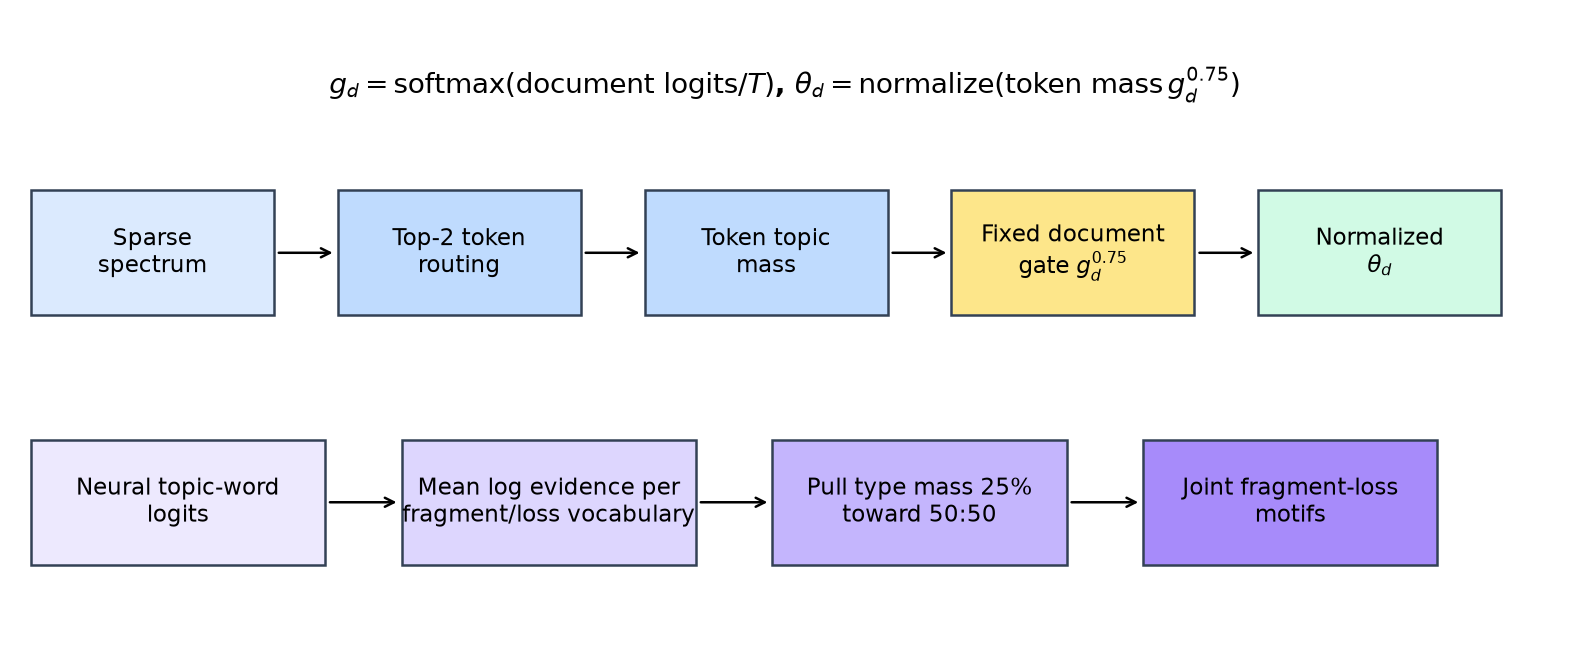
\includegraphics[width=\textwidth]{architecture.png}
  \caption{The candidate retains the fixed document gate and soft token-type
  balance, but makes fragment and neutral-loss evidence comparable by removing
  vocabulary-size bias before the channel softmax.}
  \label{fig:architecture}
\end{figure}

\clearpage
\section{Paper-aligned validation}

MAG annotation and SOS use validation spectra only. Library entries sharing a
validation or test connectivity key are excluded before retrieval. Topic
association follows the paper threshold, $\theta_{dk}\geq0.5$. SOS is averaged
over unique compounds within each topic. Eligible topics are divided into high
($>0.8$), intermediate ($0.6$--$0.8$, inclusive), and low ($<0.6$) bands.

The primary outcome is the number of high-confidence motifs with SOS at least
0.6. The unchanged checkpoint was first decoded with the new rule. Its frozen
diagnostic reached 61.0 percent coverage and validation NLL 8.5042, so the one
allowed full retraining proceeded. Acceptance then required all of the
following:
\begin{itemize}
  \item MAG annotation coverage of at least 60.7 percent;
  \item at least 148 useful high-confidence motifs;
  \item mean high-confidence SOS of at least 0.6318;
  \item validation NLL no greater than 8.5266; and
  \item finite, stable training and evaluation.
\end{itemize}

Runtime was descriptive rather than an acceptance gate. The candidate completed
in 4,720.0 seconds, below the recorded 5,571-second context threshold.

\section{Validation results}

\begingroup
\small
\setlength{\LTleft}{0pt}
\setlength{\LTright}{0pt}
\begin{longtable}{@{}>{\raggedright\arraybackslash}p{0.43\textwidth}rrr@{}}
\caption{Validation-only paper-relevant comparison.}\label{tab:comparison}\\
\toprule
Metric & Current neural & Mean-evidence neural & Tomotopy \\
\midrule
\endfirsthead
\toprule
Metric & Current neural & Mean-evidence neural & Tomotopy \\
\midrule
\endhead
Optimized motifs & 384 & 515 & 607 \\
High-confidence SOS-evaluable motifs & 42 & 252 & 206 \\
SOS high ($>0.8$) & 10 & 43 & 58 \\
SOS intermediate ($0.6$--$0.8$) & 10 & 105 & 80 \\
SOS low ($<0.6$) & 22 & 104 & 68 \\
Useful high-confidence motifs (SOS $\geq0.6$) & 20 & 148 & 138 \\
Mean high-confidence SOS & 0.6227 & 0.6418 & 0.6761 \\
Median high-confidence SOS & 0.5866 & 0.6477 & 0.6854 \\
Model-fitting time (minutes) & 84.4 & 59.5 & 76.0 \\
\bottomrule

\end{longtable}
\endgroup

\begin{figure}[ht]
  \centering
  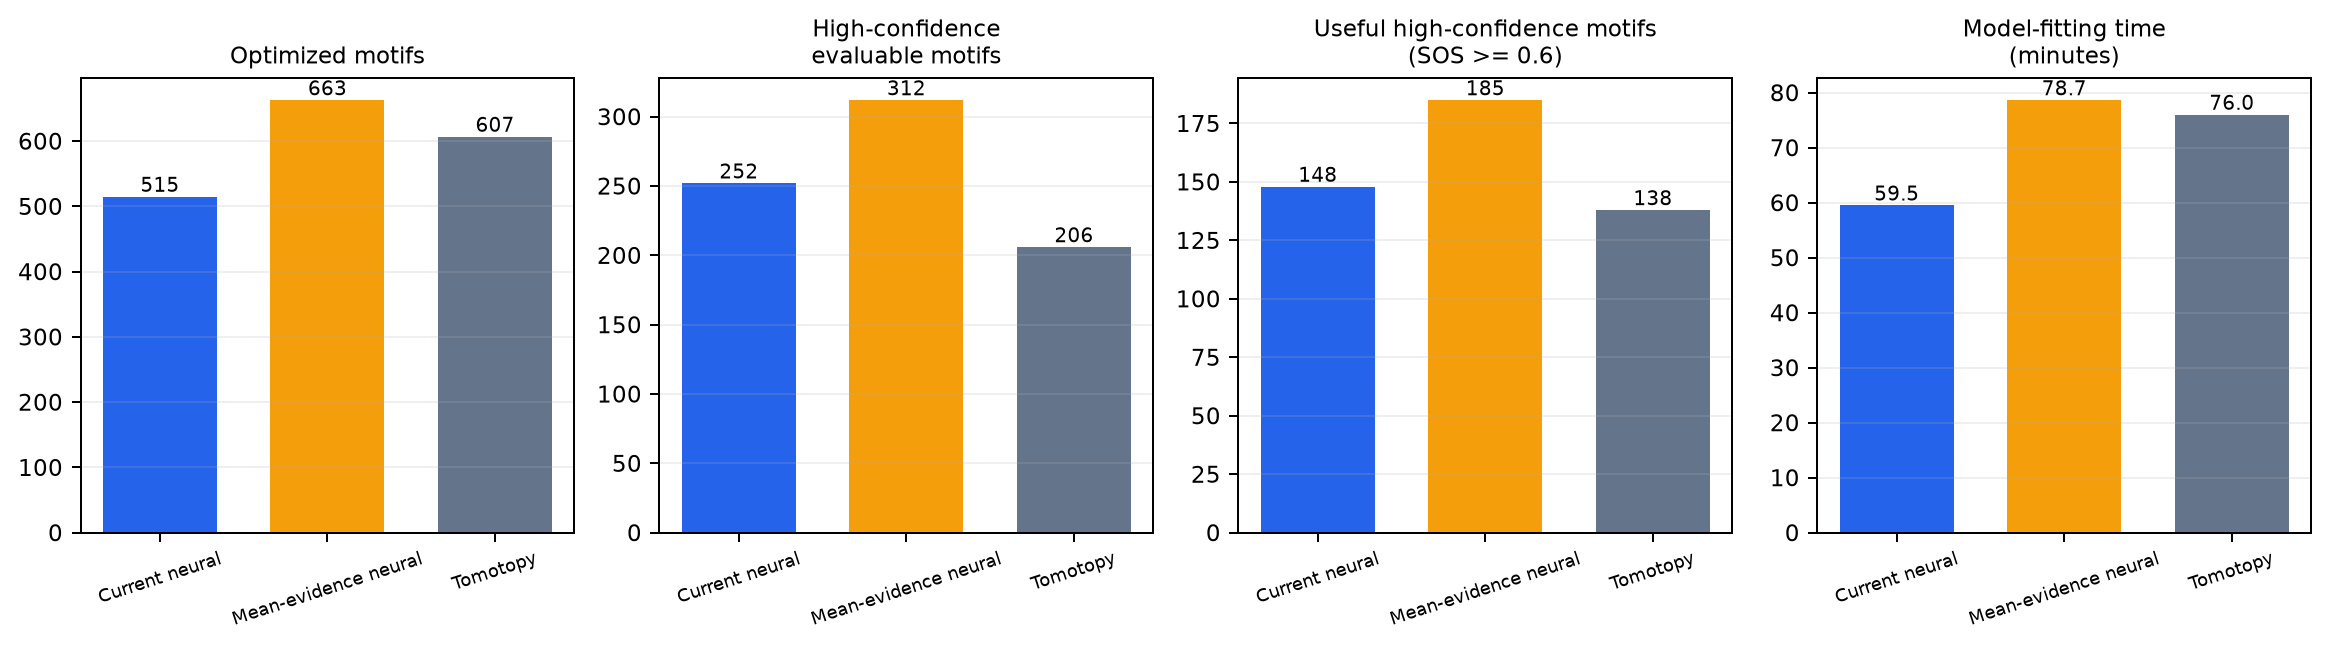
\includegraphics[width=\textwidth]{final_comparison.png}
  \caption{Headline validation outcomes and model-fitting time. The accepted
  model exceeds Tomotopy on both useful high-confidence motifs and broad MAG
  annotation coverage.}
  \label{fig:comparison}
\end{figure}

\clearpage

\begin{figure}[ht]
  \centering
  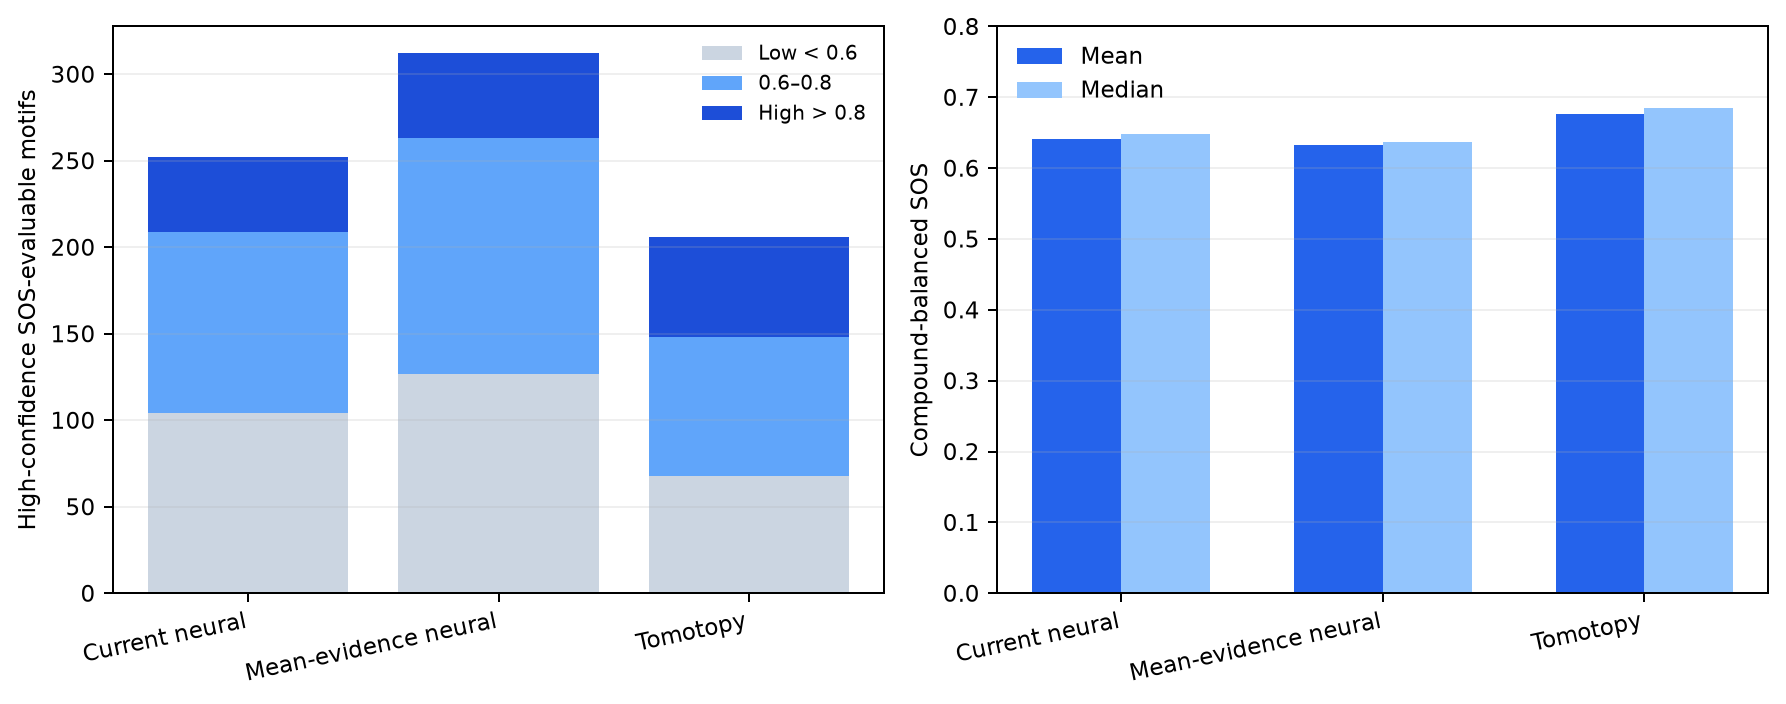
\includegraphics[width=0.94\textwidth]{chemistry_coverage.png}
  \caption{Validation high-confidence chemical evidence. Left: SOS bands among
  evaluable motifs. Right: compound-balanced mean and median SOS.}
  \label{fig:chemistry}
\end{figure}

The candidate increases annotation coverage from 515 to 663 motifs, surpassing
Tomotopy's 607. It closes 160.9 percent of the remaining 9.2-percentage-point
coverage gap. High-confidence SOS-evaluable motifs rise from 252 to 312, versus
206 for Tomotopy. Useful motifs rise from 148 to 185, 47 more than Tomotopy's
138.

Candidate mean SOS is 0.6323 versus 0.6418 for the current neural model and
0.6761 for Tomotopy. Median SOS is 0.6364, versus 0.6477 and 0.6854. This is the
declared tradeoff: much broader annotatability with a modest validation SOS
reduction that remains above the 0.6318 floor.

Validation NLL is 8.5014, only 0.0051 above the current neural 8.4963 and below
the 8.5266 safety limit. Training remains finite and stable with 321
corpus-active topics. Fitting takes 78.7 minutes, versus 59.5 minutes for the
current neural reference and 76.0 minutes for the reused Tomotopy source run.

\section{Single locked test confirmation}

All validation checks passed before the test matrices and records were linked
into the candidate run. The epoch-40 checkpoint hash was fixed, after which one
neural test inference and one leakage-filtered chemistry evaluation were
performed. No parameter changed after test access.

\begingroup
\small
\setlength{\LTleft}{0pt}
\setlength{\LTright}{0pt}
\begin{longtable}{@{}>{\raggedright\arraybackslash}p{0.56\textwidth}rr@{}}
\caption{One-time held-out test confirmation.}\label{tab:test}\\
\toprule
Metric & Mean-evidence neural & Tomotopy \\
\midrule
\endfirsthead
\toprule
Metric & Mean-evidence neural & Tomotopy \\
\midrule
\endhead
Optimized motifs & 663 & 607 \\
High-confidence SOS-evaluable motifs & 424 & 333 \\
SOS high ($>0.8$) & 58 & 66 \\
SOS intermediate ($0.6$--$0.8$) & 176 & 120 \\
SOS low ($<0.6$) & 190 & 147 \\
Useful high-confidence motifs (SOS $\geq0.6$) & 234 & 186 \\
Mean high-confidence SOS & 0.6204 & 0.6369 \\
Median high-confidence SOS & 0.6135 & 0.6145 \\
Held-out completion NLL & 8.5226 & 9.7569 \\
\bottomrule

\end{longtable}
\endgroup

The test result confirms the breadth improvement. The candidate produces 234
useful high-confidence motifs versus Tomotopy's 186 and 424 SOS-evaluable motifs
versus 333. Annotation coverage is 66.3 versus 60.7 percent. Mean SOS is lower
(0.6204 versus 0.6369), while the medians are nearly identical (0.6135 versus
0.6145). Candidate completion NLL is 8.5226 versus Tomotopy's 9.7569.

\clearpage
\section{Secondary inference context}

\begin{figure}[H]
  \centering
  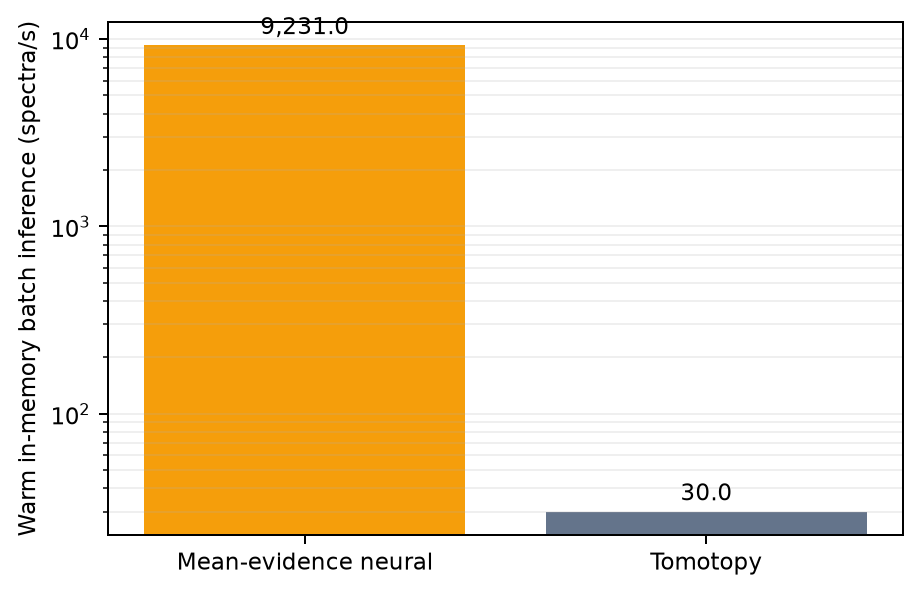
\includegraphics[width=0.68\textwidth]{inference_speed.png}
  \caption{Matched six-thread warm in-memory batch inference on the held-out
  test matrices. This secondary result is not an acceptance gate or end-to-end
  application latency.}
  \label{fig:speed}
\end{figure}

The accepted one-pass neural checkpoint processes 9,231 spectra/s in the fixed
128-spectrum warm batch, versus 30.0 spectra/s for Tomotopy with 100 inference
iterations, a 307-fold ratio. ``Warm in-memory batch inference'' means that the
model and batch are already loaded and one warm-up has completed. It is usable
for serving or repeated batches, but excludes file loading, preprocessing, and
first-call setup.

\section{Interpretation}

The remaining broad-coverage failure was a decoder accounting bias, not a need
for a larger architecture. Mean-normalizing each token type's evidence removes
that bias without a new encoder, loss, or iterative inference step. Combined
with the existing gate and soft balance, it exceeds Tomotopy on annotation
coverage and useful-motif count on validation and test while maintaining much
better predictive fit.

The remaining weakness is SOS strength: broader candidate coverage includes
more low-SOS topics, and test mean SOS is 0.0165 below Tomotopy. This is a clear
tradeoff rather than evidence that every candidate motif is superior. The result
remains one fixed-seed architecture experiment. Replication across seeds is a
separate confirmation stage, and no claim is made that this research checkpoint
replaces the production Tomotopy backend.

\section{Reproducibility}

The report retains the resolved comparison summary and hashed source manifests
for training, all validation references, the gate decision, the test-access
record, and both test evaluations. The candidate checkpoint is fixed at epoch
40 with SHA-256:
\begin{center}
\small\texttt{639c1f37c613d908b59e3a85b7dc701e}\\[-2pt]
\texttt{33a3f92fd7476a3257b47298143dfbc6}
\end{center}
The test-access manifest confirms that selection was final before test.

\begin{thebibliography}{9}
\bibitem{vanderhooft2016}
J. J. J. van der Hooft et al. ``Topic modeling for untargeted substructure
exploration in metabolomics.'' \emph{Proceedings of the National Academy of
Sciences}, 2016.
\url{https://pmc.ncbi.nlm.nih.gov/articles/PMC5137707/}

\bibitem{ms2lda2026}
M. Torres Ortega et al. ``Large-scale discovery and annotation of substructure
patterns in mass spectrometry profiles.'' \emph{Nature Communications}, 2026.
\url{https://www.nature.com/articles/s41467-026-75038-0}
\end{thebibliography}

\end{document}
